%% ICTC 2026 — IWETRIAI (ETRI Human Understanding AI Paper Challenge)
%% IEEE conference template, 4-page full paper.
%% Compile on Overleaf with pdfLaTeX. Figures in ./figs (generated by make_figs.py).
\documentclass[conference]{IEEEtran}
\IEEEoverridecommandlockouts
\usepackage{cite}
\usepackage{amsmath,amssymb,amsfonts}
\usepackage{graphicx}
\usepackage{booktabs}
\usepackage{textcomp}
\usepackage{xcolor}
\usepackage{url}
\def\BibTeX{{\rm B\kern-.05em{\sc i\kern-.025em b}\kern-.08em T\kern-.1667em\lower.7ex\hbox{E}\kern-.125emX}}

\begin{document}

\title{Validation Reliability, Not Model Capacity, Is the Bottleneck:\\
A Shift-Aware Multi-Source Ensemble for Sleep-Metric Prediction\\
from Consumer Lifelog Sensors}

\author{
\IEEEauthorblockN{Donghyun Seo}
\IEEEauthorblockA{\textit{Independent Researcher}\\
Republic of Korea \\
tjehdgus113@gmail.com}
}

\maketitle

\begin{abstract}
We study the prediction of seven binary nightly sleep metrics from a single
preceding day of consumer smartphone and smartwatch sensor logs, as posed by the
ETRI 2026 Human Understanding AI Challenge. The task couples two difficulties that
are common in real lifelog settings but rarely addressed together: a very small
sample ($N{=}450$ training nights over only ten subjects) and a \emph{temporal
distribution shift}, where the evaluation nights fall predominantly later in time
than the training nights. We build a nine-source ensemble spanning gradient-boosted
trees, sequence neural networks, a frozen vision foundation model, an actigraphy-style
sleep reconstruction, and a label-autocorrelation neighbour model, combined by
per-target greedy blending. Our central finding is methodological: under temporal
shift and small $N$, the binding constraint is not model capacity but
\emph{validation reliability}. Random $k$-fold cross-validation systematically
rewards changes that fail to generalize, whereas only two classes of improvement
transfer to held-out data---multi-seed variance reduction and \emph{forward-chaining
(shift-aware) reweighting}. Our final submission attains an Average Log-Loss of $0.578$; more importantly,
controlled ablations show that disciplined, shift-aware validation---rather than added
model capacity---is what produced the improvements that generalized. We further give an
honest analysis of the resulting data ceiling, which is structural: four of the seven
labels derive from a clinical sleep sensor that is absent from the inputs.
\end{abstract}

\begin{IEEEkeywords}
lifelog, sleep prediction, ensemble learning, distribution shift, time-series
cross-validation, small-sample learning
\end{IEEEkeywords}

\section{Introduction}
Consumer wearables and smartphones passively record rich behavioural and
physiological signals, raising the prospect of inferring sleep quality from everyday
devices rather than dedicated clinical hardware. The ETRI 2026 Human Understanding AI
Challenge formalizes one such task: given a single day of twelve passively logged
sensor streams, predict seven binary descriptors of \emph{that night's} sleep. Three
descriptors (Q1--Q3) are subjective survey outcomes---sleep quality, fatigue, and
stress---each binarized \emph{relative to the individual's own long-run average}. The
remaining four (S1--S4) encode whether the night met National Sleep Foundation (NSF)
guidelines on total sleep time, sleep efficiency, sleep-onset latency, and wake after
sleep onset~\cite{nsf}.

Two properties make the task unusually treacherous. First, the data are
\emph{small}: 450 training nights drawn from only ten subjects, with 250 evaluation
nights from the same individuals. Second, there is a \emph{temporal shift}: the
evaluation nights lie largely after the training window for each subject
(Fig.~\ref{fig:shift}). Together these mean that a model can easily memorize
subject-specific idiosyncrasies, and---more dangerously---that a naive validation
estimate computed by randomly shuffling nights will be \emph{optimistically biased}
relative to the genuinely forward-in-time evaluation set.

The scoring metric is the macro (label-averaged) logarithmic loss,
\begin{equation}
\mathcal{L} = \frac{1}{7}\sum_{j=1}^{7}
-\frac{1}{N}\sum_{i=1}^{N}\Big[y_{ij}\log \hat p_{ij}+(1-y_{ij})\log(1-\hat p_{ij})\Big],
\label{eq:logloss}
\end{equation}
which rewards \emph{calibrated probabilities} and punishes confident mistakes far
more than a plain accuracy score would. Lower is better.

Our contributions are threefold:
\begin{itemize}
\item A diverse nine-source ensemble for consumer-sensor sleep-metric prediction,
including an actigraphy-style sleep reconstruction that directly targets the
NSF labels and a frozen vision-model embedding that injects an orthogonal view of
the sensor time series (Section~\ref{sec:method}).
\item The empirical observation, made the centrepiece of the paper, that under
temporal shift and small $N$ the operative bottleneck is \emph{validation
reliability}: random-fold cross-validation misleads, and only variance reduction
and forward-chaining reweighting transfer to held-out data
(Sections~\ref{sec:exp}--\ref{sec:disc}).
\item An honest characterization of the structural data ceiling that bounds achievable
performance on this task, rooted in a clinical modality absent from the inputs
(Section~\ref{sec:disc}).
\end{itemize}

\section{Data and Problem Setting}
\label{sec:data}
Each night is associated with a \texttt{lifelog\_date} (the preceding day whose
sensors are observed) and a \texttt{sleep\_date}. Twelve sensor families are
provided: heart rate and pedometer from the watch; screen, charging, activity-state,
ambient-sound, GPS, light, Wi-Fi, BLE, and app-usage from the phone. Sampling and
coverage vary widely; the watch heart-rate stream in particular stores per-timestamp
\emph{arrays} of sub-second readings and is the sparsest at night.

\paragraph{Label structure} The two label families demand different inductive
biases. Because Q1--Q3 are defined relative to a personal mean, their positive rate
varies strongly across subjects (ranging roughly from $0.15$ to $0.85$ depending on
subject and label); this motivates \emph{within-subject normalization} of features and
a ranking-based treatment of the Q targets. By contrast S1--S4 use \emph{absolute} clinical thresholds, so a
subject's compliance rate is comparatively stable, and a per-subject base-rate prior
is a strong anchor.

\paragraph{The missing modality} Critically, S1--S4 are computed from a Withings
Sleep Analyzer---a bedside device that is \emph{not} among the twelve input streams.
The phone and watch can only \emph{proxy} the quantities (total sleep time, efficiency,
latency, wake) that those labels threshold. This gap is the source of the structural
ceiling we report in Section~\ref{sec:disc}.

\paragraph{Temporal shift} Fig.~\ref{fig:shift} plots \texttt{sleep\_date} for the
training and evaluation nights per subject. For every subject the evaluation nights
(orange) extend beyond the training nights (green). A validation protocol that
shuffles nights uniformly therefore evaluates on a distribution the deployed model
will never see; we return to this in Section~\ref{sec:method}.

\begin{figure}[t]
\centering
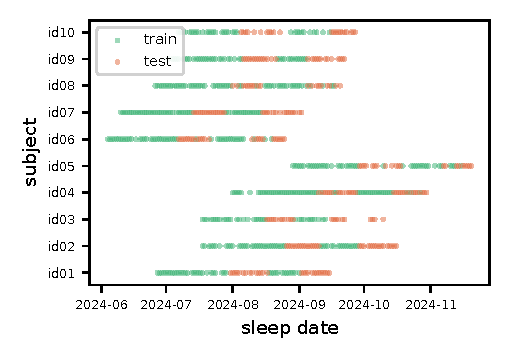
\includegraphics[width=\columnwidth]{figs/shift.pdf}
\caption{Per-subject temporal distribution of training (green) and evaluation
(orange) nights. Evaluation nights fall consistently later in time, defining the
distribution shift the model must survive. This single observation motivates the
forward-chaining validation of Section~\ref{sec:method}.}
\label{fig:shift}
\end{figure}

\section{Method}
\label{sec:method}
Our system follows a three-stage structure: (i) build several diverse base sources,
(ii) combine them per target by greedy blending, and (iii) apply shift- and
definition-aware corrections. All features are normalized within subject so that they
encode ``today relative to this person's habit,'' matching the relative definition of
the Q labels.

\subsection{Feature engineering}
Each sensor is aggregated to one row per (subject, \texttt{lifelog\_date}) over named
hour windows (e.g.\ daytime, evening, pre-bed, night, morning) with the usual
order statistics, plus night windows attributed to the correct calendar night. On top
of the daily table we add per-subject temporal derivatives---lagged differences,
rolling and exponential means, and an expanding mean---to encode personal baselines.
The watch heart-rate arrays are reduced to per-minute mean/min/max/std after removing
physiologically implausible values.

\subsection{Base sources}
We construct nine sources chosen for \emph{mechanistic diversity}:
\begin{enumerate}
\item \textbf{Tree.} A weighted average of LightGBM~\cite{lightgbm},
CatBoost~\cite{catboost} and Extremely Randomized Trees, with ExtraTrees importances
selecting the top 150 features and a pseudo-labeling pass (confidence threshold $0.85$)
that adds high-confidence evaluation rows to training.
\item \textbf{Prior.} The per-subject historical label mean---a simple but strong
anchor, especially for the absolute S labels.
\item \textbf{Sequence networks (GRU, BiLSTM, TCN~\cite{tcn}, Attention).} Each is a
small 1-D CNN encoder followed by the respective sequence module, a subject embedding,
and a shared seven-head output. Each architecture is trained with eight random seeds
and \emph{averaged} (we call this \emph{DLens}); since neural networks are
high-variance learners on $N{=}450$, seed averaging reduces variance in the spirit of
weight averaging~\cite{swa}.
\item \textbf{Vision embedding (SigLIP-Large).} The sensor series are rendered as 2-D
images and passed through a \emph{frozen} SigLIP-Large vision
transformer~\cite{siglip}; the pooled embeddings feed a gradient-boosted model. The
weights are never trained---the model supplies a generic visual encoding that is
orthogonal to the tree and sequence views.
\item \textbf{Sleep reconstruction (SleepTree2).} An actigraphy-style routine
reconstructs the main sleep episode from nocturnal movement, heart rate, and charging,
yielding minute-level estimates of total sleep time, efficiency, latency and wake plus
NSF-threshold flags; these feed a tree model and directly target S1--S4.
\item \textbf{Neighbour.} An exponentially date-weighted average of the same subject's
\emph{other} nights' labels (computed leave-one-out), exploiting the autocorrelation
of sleep outcomes across nearby dates.
\end{enumerate}
We additionally compute a label-free \emph{day-state} representation by a transductive
non-negative matrix factorization~\cite{nmf} of 30-minute behaviour bins over all 700
days, used to route the Q1/Q2 predictions.

\subsection{Blending}
For each target we select source weights by greedy coordinate descent, starting from
the prior anchor and adjusting weights in $\pm 0.05/0.10$ steps to minimize
(\ref{eq:logloss}). Fig.~\ref{fig:srcll} shows that no single source dominates all
labels---the sleep reconstruction is strongest on several S targets, the neighbour
model on a Q target---which is precisely the condition under which blending pays.

\subsection{Definition- and shift-aware corrections}
Two corrections embody the paper's thesis that the right inductive bias matters more
than raw capacity.

\paragraph{Pairwise ranking for Q} Because the Q labels are defined by comparison to a
personal average, we additionally learn a \emph{pairwise} ranker~\cite{ranknet}: for
each subject we form (positive-night, negative-night) pairs and fit a ridge logistic
model on their feature differences, adding the result as a scaled residual
($\alpha{=}0.15$ in logit space) to Q1/Q2.

\paragraph{Forward-chaining reweighting for S} This is the key lever. The blend
weights above are chosen on randomly shuffled folds, which---as
Fig.~\ref{fig:shift} warns---do not reflect the forward-in-time evaluation set. We
therefore re-select the S1/S4 weights using \emph{forward-chaining} folds: using the
earliest $0.5$ to $0.8$ of nights for training, each fold validates on the following
$20\%$ block, sliding the split forward~\cite{bergmeir}. Fig.~\ref{fig:forward} shows that the forward protocol moves
weight away from sources that look good only in-sample and toward sources that are
robust to the shift. As we report next, this is one of only two changes that transfer
to held-out performance.

\begin{figure}[t]
\centering
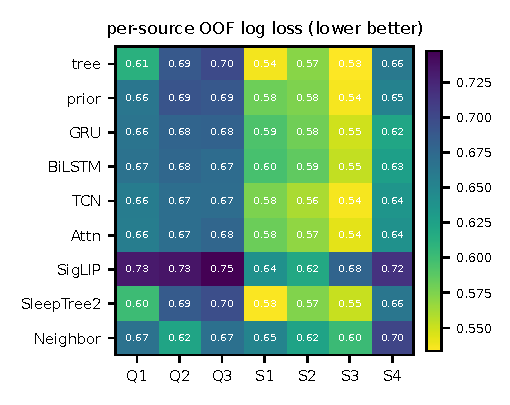
\includegraphics[width=\columnwidth]{figs/srcll.pdf}
\caption{Out-of-fold log loss of each base source per label (lighter is better). No
source dominates every target, justifying the per-target blend.}
\label{fig:srcll}
\end{figure}

\begin{figure*}[t]
\centering
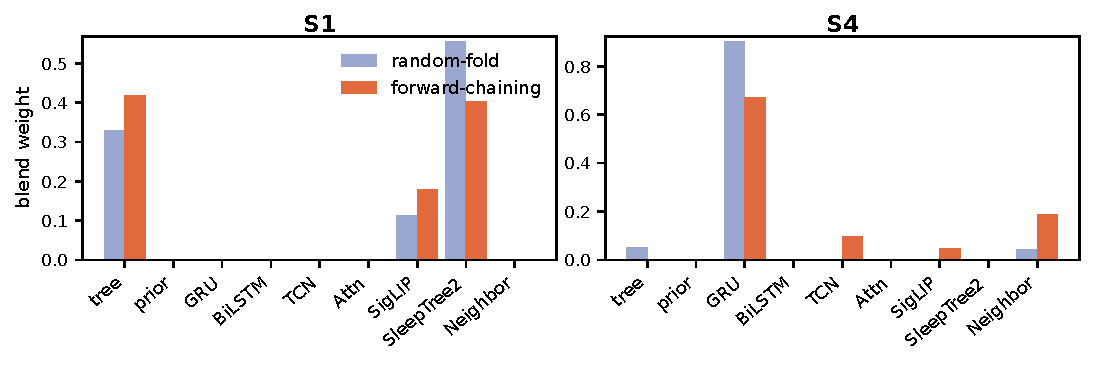
\includegraphics[width=0.92\textwidth]{figs/forward.pdf}
\caption{Blend weights for S1 and S4 chosen by random-fold (blue) versus
forward-chaining (orange) validation over the same nine sources. The shift-aware
protocol redistributes weight toward sources that generalize forward in time (e.g.,
on S4 away from the in-sample-favoured GRU toward TCN and the neighbour model); this
reweighting is the single largest source of held-out improvement.}
\label{fig:forward}
\end{figure*}

\section{Experiments}
\label{sec:exp}
We report the macro log loss (\ref{eq:logloss}); lower is better, with a chance-level
predictor at $0.693$. We use internal out-of-fold (OOF) cross-validation during
development and the challenge's held-out test leaderboard for final evaluation. Our
nine-source backbone scores $0.584$ in OOF; adding the definition- and shift-aware
corrections of Section~\ref{sec:method} yields a final held-out \emph{Average Log-Loss
of $0.578$}. Because an absolute score is only meaningful against this particular
benchmark, our analysis emphasizes \emph{relative} comparisons, which are far more
informative about what actually generalizes.

\paragraph{What transferred} Table~\ref{tab:transfer} summarizes the two improvements
that moved the held-out score and contrasts them with a representative ``illusory''
change. Multi-seed DLens averaging gave a small but reliable gain. The forward-chaining
reweighting of S1/S4 was the largest single lever; held-out performance improved
monotonically as we strengthened its influence. In contrast, candidates that diverged
substantially from the current best prediction---even when they improved the
random-fold OOF estimate---consistently \emph{worsened} the held-out score, a pattern
we observed repeatedly across roughly twenty tested ideas.

\begin{table}[t]
\caption{Improvements that transfer to held-out data are exactly those that reduce
variance or respect the temporal shift; changes that merely improve a random-fold
estimate do not transfer.}
\label{tab:transfer}
\centering
\small
\begin{tabular}{@{}lcc@{}}
\toprule
Change & Random-fold OOF & Held-out \\
\midrule
Multi-seed averaging (DLens)        & improves & improves (small) \\
Forward-chaining S1/S4 reweighting  & --       & \textbf{improves (largest)} \\
High-divergence ``new-signal'' edits & improves & worsens \\
\bottomrule
\end{tabular}
\end{table}

\paragraph{Source diversity} Diversity is what makes the blend pay. While the four
sequence networks are, as expected, mutually correlated (up to $0.98$), the
mechanistically distinct families---trees, sleep reconstruction, neighbour, and the
frozen vision embedding---are decorrelated to as low as $0.24$ in their predictions.
It is this \emph{cross-family} disagreement, rather than within-family redundancy,
that the per-target blend exploits, and it explains why the blend outperforms every
individual source despite each source being weaker on its own.

\section{Discussion}
\label{sec:disc}

\paragraph{Why random CV misleads here} The combination of small $N$, only ten
subjects, and a forward-in-time evaluation set means a randomly shuffled fold leaks
information in two ways: nearby nights of the same subject are highly autocorrelated,
and the fold never reproduces the temporal gap the model faces at test time.
Consequently the random-fold estimate rewards subtle overfitting. Forward-chaining
validation removes the second leak and tracks held-out behaviour far better; it is the
discipline, not a new feature, that produced our gains.

\paragraph{The structural ceiling} Despite extensive search---vision models, multiple
sleep-reconstruction variants, heart-rate-variability textures, per-subject models,
external weather and connectivity features, and several label-structure
exploits---no ``big bet'' produced a held-out gain once validated without leakage.
The reason is structural: S1--S4 threshold quantities measured by a clinical device
absent from the inputs, and Q2--Q3 are subjective states only loosely determined by
behaviour. The phone and watch can proxy these only so far, which bounds the
achievable score. We regard the honest demarcation of this ceiling as a useful
negative result for the lifelog community.

\section{Conclusion}
\label{sec:conc}
For nightly sleep-metric prediction from consumer lifelog sensors under small samples
and temporal shift, we found that the decisive factor was not model capacity but the
reliability of the validation protocol. A mechanistically diverse nine-source ensemble
provided a strong backbone, but the improvements that actually generalized were those
that reduced variance (seed averaging) or respected the temporal shift
(forward-chaining reweighting); changes that merely improved a random-fold estimate
did not transfer. We additionally documented a structural data ceiling rooted in a
missing clinical modality. We hope these observations help practitioners working with
similarly small, shifted lifelog datasets prioritize honest validation over added
capacity.

\section*{Acknowledgment}
The authors thank the ETRI 2026 Human Understanding AI Challenge organizers for the
dataset and evaluation infrastructure.

\begin{thebibliography}{00}
\bibitem{nsf} M. Hirshkowitz \emph{et al.}, ``National Sleep Foundation's sleep time
duration recommendations: methodology and results summary,'' \emph{Sleep Health},
vol.~1, no.~1, pp.~40--43, 2015.
\bibitem{lightgbm} G. Ke \emph{et al.}, ``LightGBM: A highly efficient gradient
boosting decision tree,'' in \emph{Adv. Neural Inf. Process. Syst. (NeurIPS)}, 2017.
\bibitem{catboost} L. Prokhorenkova \emph{et al.}, ``CatBoost: unbiased boosting with
categorical features,'' in \emph{Adv. Neural Inf. Process. Syst. (NeurIPS)}, 2018.
\bibitem{tcn} S. Bai, J. Z. Kolter, and V. Koltun, ``An empirical evaluation of
generic convolutional and recurrent networks for sequence modeling,''
\emph{arXiv:1803.01271}, 2018.
\bibitem{swa} P. Izmailov \emph{et al.}, ``Averaging weights leads to wider optima and
better generalization,'' in \emph{Proc. Conf. Uncertainty in Artificial Intelligence
(UAI)}, 2018.
\bibitem{siglip} X. Zhai, B. Mustafa, A. Kolesnikov, and L. Beyer, ``Sigmoid loss for
language image pre-training,'' in \emph{Proc. IEEE/CVF Int. Conf. Comput. Vis.
(ICCV)}, 2023.
\bibitem{ranknet} C. Burges \emph{et al.}, ``Learning to rank using gradient
descent,'' in \emph{Proc. Int. Conf. Machine Learning (ICML)}, 2005.
\bibitem{bergmeir} C. Bergmeir and J. M. Ben\'itez, ``On the use of cross-validation
for time series predictor evaluation,'' \emph{Information Sciences}, vol.~191,
pp.~192--213, 2012.
\bibitem{nmf} D. D. Lee and H. S. Seung, ``Learning the parts of objects by
non-negative matrix factorization,'' \emph{Nature}, vol.~401, pp.~788--791, 1999.
\end{thebibliography}

\end{document}
